\documentclass[referat]{SCWorks}
\usepackage{preamble}
\setminted[py]{fontsize=\small, breaklines=true, style=bw, linenos}
\newcommand{\eqdef}{\stackrel {\rm def}{=}}
\newcommand{\specialcell}[2][c]{%
    \begin{tabular}[#1]{@{}c@{}}#2\end{tabular}}

\usepackage{forest}

\renewcommand\theFancyVerbLine{\small\arabic{FancyVerbLine}}

\newtheorem{lem}{Лемма}
\linespread{1.5}
\setminted{
    fontsize=\small,          % Размер шрифта
    baselinestretch=1.0,      % Единичный интервал
    breaklines=true,          % Перенос строк
    framesep=2mm,             % Отступ вокруг кода
    linenos=false,            % Нумерация строк (опционально)
    xleftmargin=2em,          % Отступ слева
    breakanywhere=true,
}
\begin{document}
    \studentfemale

    \chair{информатики и программирования}

    \title{отчет по графам}

    \course{3}

    \group{341}

    \napravlenie{02.03.01 "--- Математическое обеспечение и администрирование информационных систем}

    \studenttitle{студентки}

    \author{Загудалиной Вероники Павловны}

    \chtitle{доцент, к.\,ф.-м.\,н.}
    \chname{М.\,В.\,Огнева}

    \satitle{доцент, к.\,п. н.}
    \saname{А.\,А.\,Казачкова}

    \term{5}

    \practtype{отчет по графам}

    \date{2026}

    \maketitle

    \secNumbering

    \tableofcontents


    \section{Минимальные требования для класса Граф}

    \subsection{Условие}
    Для решения всех задач курса необходимо создать класс (или иерархию классов - на усмотрение разработчика), содержащий:

    1. Структуру для хранения списка смежности графа (не работать с графом через матрицы смежности, если в некоторых алгоритмах удобнее использовать список ребер - реализовать метод, создающий список рёбер на основе списка смежности);

    2. Конструкторы (не менее 3-х):



    \begin{itemize}
        \item конструктор по умолчанию, создающий пустой граф

        \item конструктор, заполняющий данные графа из файла

        \item конструктор-копию (аккуратно, не все сразу делают именно копию)

        \item специфические конструкторы для удобства тестирования
    \end{itemize}
    3. Методы:



    \begin{itemize}
        \item добавляющие вершину,

        \item добавляющие ребро (дугу),

        \item удаляющие вершину,

        \item удаляющие ребро (дугу),
        \item выводящие список смежности в файл (в том числе в пригодном для чтения конструктором формате).
    \end{itemize}
    Не выполняйте некорректные операции, сообщайте об ошибках.


    4. Должны поддерживаться как ориентированные, так и неориентированные графы.
    Заранее предусмотрите возможность добавления меток и\\или весов для дуг.
    Поддержка мультиграфа не требуется.

    5. Добавьте минималистичный \textbf{консольный} интерфейс пользователя (не смешивая его с реализацией!), позволяющий добавлять и удалять вершины и рёбра (дуги) и просматривать текущий список смежности графа.

    6. Сгенерируйте не менее 4 входных файлов с разными типами графов (балансируйте на комбинации ориентированность-взвешенность) для тестирования класса в этом и последующих заданиях. Графы должны содержать не менее 7-10 вершин, в том числе петли и изолированные вершины.


    Замечание:

    В зависимости от выбранного способа хранения графа могут появиться дополнительные трудности при удалении-добавлении, например, необходимость переименования вершин, если граф хранится списком (например, vector C++, List C#). Этого можно избежать, если хранить в списке пару (имя вершины, список смежных вершин), или хранить в другой структуре (например, Dictionary C#, map в С++, при этом список смежности вершины может также храниться в виде словаря с ключами - смежными вершинами и значениями - весами соответствующих ребер). Идеально, если в качестве вершины реализуется обобщенный тип (generic), но достаточно использовать строковый тип или свой класс.


    \subsection{Реализация}

    \begin{itemize}
        \item \textbf{Структура данных}: Для хранения используется словарь словарей
        \verb|self._adj_list = { vertex: {neighbor: weight} }|.
        Это обеспечивает быстрый доступ к соседям и весам ребер ($O(1)$ в среднем).


        \item \textbf{Универсальность}: Ориентированность управляется флагом \verb|is_directed|.
        Если он False, то при добавлении ребра $(u, v)$ программа автоматически добавляет обратное ребро $(v, u)$.


        \item \textbf{Конструкторы}:

        \begin{itemize}
            \item \_\_init\_\_: создает пустой граф.


            \item from\_json: использует библиотеку json для десериализации данных из файла.


            \item from\_copy: реализует глубокое копирование через copy.deepcopy.


            \item from\_random: генерирует случайные связи между заданным количеством вершин.


        \end{itemize}

        \item \textbf{Интерфейс}: Реализован в классе GraphInterface по принципу разделения логики и представления. Используется система вложенных меню для управления графом.


    \end{itemize}
    Пример кода:
    \begin{minted}{text}
import copy
import json
import random
import os
import networkx as nx
import matplotlib.pyplot as plt


class GraphError(Exception):
    """Базовый класс для ошибок в работе с графом."""
    pass


class Graph:
    def __init__(self, is_directed: bool = False, is_weighted: bool = False):
        """1. Конструктор по умолчанию."""
        self.is_directed = is_directed
        self.is_weighted = is_weighted
        self._adj_list = {}

    @classmethod
    def from_json(cls, filename: str):
        """Загрузка графа из JSON файла."""
        path = "data/" + filename + ".json"
        if not os.path.exists(path):
            raise FileNotFoundError(f"Файл {filename} не найден.")

        with open(path, 'r', encoding='utf-8') as f:
            data = json.load(f)

        instance = cls(is_directed=data['is_directed'], is_weighted=data['is_weighted'])
        instance._adj_list = data['adj_list']
        return instance

    @classmethod
    def from_copy(cls, other):
        """3. Конструктор-копия."""
        if not isinstance(other, Graph):
            raise TypeError("Копируемый объект должен быть экземпляром класса Graph.")

        instance = cls(other.is_directed, other.is_weighted)
        instance._adj_list = copy.deepcopy(other._adj_list)
        return instance

    @classmethod
    def from_random(cls, num_vertices: int, num_edges: int, is_directed: bool = False, is_weighted: bool = False):
        """4. Специфический конструктор для генерации случайного графа."""
        if num_vertices <= 0:
            raise ValueError("Количество вершин должно быть положительным.")

        max_possible_edges = num_vertices * num_vertices if is_directed else (num_vertices * (num_vertices + 1)) // 2
        if num_edges > max_possible_edges:
            raise GraphError(f"Слишком много ребер ({num_edges}) для {num_vertices} вершин.")

        instance = cls(is_directed, is_weighted)
        vertices = [f"V{i}" for i in range(1, num_vertices + 1)]

        for v in vertices:
            instance.add_vertex(v)

        added_edges = 0
        while added_edges < num_edges:
            u = random.choice(vertices)
            if is_directed:
                v = random.choice(vertices)
            else:
                other_vertices = [v for v in vertices if v != u]
                v = random.choice(other_vertices)

            if v not in instance._adj_list[u]:
                weight = round(random.uniform(1.0, 10.0), 1) if is_weighted else 1.0
                instance.add_edge(u, v, weight)
                added_edges += 1

        return instance

    def get_edge_list(self):
        """Возвращает список ребер в формате (откуда, куда, вес)."""
        edges = []
        visited = set()
        for u in self._adj_list:
            for v, weight in self._adj_list[u].items():
                edge_id = (u, v) if self.is_directed else tuple(sorted((u, v)))
                if self.is_directed or edge_id not in visited:
                    edges.append((u, v, weight))
                    visited.add(edge_id)
        return edges

    def add_vertex(self, v: str):
        """Добавляет вершину в граф."""
        if v in self._adj_list:
            raise GraphError(f"Вершина '{v}' уже существует.")
        self._adj_list[v] = {}

    def add_edge(self, u: str, v: str, weight: float = 1.0):
        """Добавляет ребро (дугу) между u и v."""
        if u not in self._adj_list:
            raise GraphError(f"Вершины '{u}' не существует.")
        if v not in self._adj_list:
            raise GraphError(f"Вершины '{v}' не существует.")

        if not self.is_directed and u == v:
            raise GraphError(f"В неориентированном графе не должно быть петель")

        if v in self._adj_list[u]:
            raise GraphError(f"Ребро из '{u}' в '{v}' уже существует.")

        self._adj_list[u][v] = weight
        if not self.is_directed:
            if u != v:
                self._adj_list[v][u] = weight

    def change_weight(self, u: str, v: str, weight: float = 1.0):
        if not self.is_weighted:
            raise GraphError(f"Граф невзвешенный, весов нет!")
        if u not in self._adj_list:
            raise GraphError(f"Вершины '{u}' не существует.")
        if v not in self._adj_list:
            raise GraphError(f"Вершины '{v}' не существует.")

        self._adj_list[u][v] = weight

    def remove_edge(self, u: str, v: str):
        """Удаляет ребро (дугу) из u в v."""
        if u not in self._adj_list:
            raise GraphError(f"Вершина '{u}' не найдена.")
        if v not in self._adj_list:
            raise GraphError(f"Вершина '{v}' не найдена.")
        if v not in self._adj_list[u]:
            raise GraphError(f"Ребро из '{u}' в '{v}' не найдено.")

        del self._adj_list[u][v]

        if not self.is_directed:
            if v in self._adj_list and u in self._adj_list[v]:
                del self._adj_list[v][u]

    def remove_vertex(self, v: str):
        """Удаляет вершину и все инцидентные ей ребра."""
        if v not in self._adj_list:
            raise GraphError(f"Вершина '{v}' не найдена.")

        del self._adj_list[v]

        for source, neighbors in self._adj_list.items():
            if v in neighbors:
                del neighbors[v]

    def to_json(self, filename: str):
        """Сохранение графа в JSON файл."""

        data = {
            "is_directed": self.is_directed,
            "is_weighted": self.is_weighted,
            "adj_list": self._adj_list
        }

        with open("data/" + filename + ".json", 'w', encoding='utf-8') as f:
            json.dump(data, f, ensure_ascii=False, indent=4)

    def __str__(self) -> str:
        """Пользовательское представление графа (список смежности)."""
        if not self._adj_list:
            return "Граф пуст."

        lines = []
        for u, neighbors in self._adj_list.items():
            if not neighbors:
                lines.append(f"{u}: -")
            else:
                neighbor_parts = []
                for v, w in neighbors.items():
                    part = f"{v}({w})" if self.is_weighted else str(v)
                    neighbor_parts.append(part)

                lines.append(f"{u}: {', '.join(neighbor_parts)}")
        return "\n".join(lines)

    def __repr__(self) -> str:
        """Техническое представление графа."""
        return f"Graph({"ориентированный" if self.is_directed else "неориентированный"}, {"взвешенный" if self.is_weighted else "невзвешенный"}, количество вершин={len(self._adj_list)})"

    def visualize(self):
        """ Визуализирует граф """

        nx_graph = nx.DiGraph() if self.is_directed else nx.Graph()
        nx_graph.add_nodes_from(self._adj_list.keys())
        for u, neighbors in self._adj_list.items():
            for v, weight in neighbors.items():
                nx_graph.add_edge(u, v, weight=weight)

        pos = nx.spring_layout(nx_graph, k=2.0, iterations=50)

        plt.figure(figsize=(10, 7))

        nx.draw_networkx_nodes(nx_graph, pos, node_size=1300, node_color='lightblue')

        nx.draw_networkx_labels(nx_graph, pos, font_size=10, font_family='sans-serif', font_weight='bold')

        if self.is_directed:
            nx.draw_networkx_edges(
                nx_graph, pos,
                edgelist=nx_graph.edges(),
                arrowstyle='->',
                arrowsize=30,
                edge_color='gray',
                width=2,
                node_size=1500,
                connectionstyle='arc3, rad=0.1'
            )
        else:
            nx.draw_networkx_edges(nx_graph, pos, width=2, edge_color='gray')

        if self.is_weighted:
            edge_labels = nx.get_edge_attributes(nx_graph, 'weight')

            if self.is_directed:
                nx.draw_networkx_edge_labels(
                    nx_graph, pos,
                    edge_labels=edge_labels,
                    label_pos=0.3,
                    font_size=9,
                    rotate=True,
                    bbox=dict(facecolor='white', edgecolor='none', alpha=0.6, boxstyle='round,pad=0.2')
                )
            else:
                nx.draw_networkx_edge_labels(
                    nx_graph, pos,
                    edge_labels=edge_labels,
                    font_size=9
                )

        plt.title(f"Визуализация: {'Ориентированный' if self.is_directed else 'Неориентированный'} граф")
        plt.axis('off')
        plt.tight_layout()
        plt.show()

    \end{minted}

    \subsection{Пример работы}
    \begin{minted}{json}
{
    "is_directed": false,
    "is_weighted": true,
    "adj_list": {
        "A": {"B": 5, "C": 10},
        "B": {"A": 5, "D": 3},
        "C": {"A": 10},
        "D": {"B": 3}
    }
}
    \end{minted}


    Примечание: в меню уже добавлены пункты, которые выполняли задания, которые были выданы на практике.
    \begin{minted}{text}
--- Система управления графами ---

--- СОЗДАНИЕ ---
1. Создать пустой
2. Создать из json
3. Сгенерировать новый случайный
4. Объединить 2 графа из json
5. Объединить текущий с другим (из json)
0. Выход
> 2
Имя файла: aboba
Загружено.

==============================
 ТЕКУЩИЙ ГРАФ: Graph(неориентированный, взвешенный, количество вершин=4)
==============================
1. [Создание] (Начать заново / Сгенерировать другой)
2. [Редактирование] (Вершины / Ребра)
3. [Просмотр] (Список смежности / Рисунок)
4. [Алгоритмы путей] (Йен, Флойд, Беллман, Эдмондс-Карп)
5. [Файлы] (Сохранить результат)
0. Выход

Выберите категорию: 3

--- ПРОСМОТР ---
1. Список смежности
2. Визуализация
3. Степени всех вершин
4. Найти не смежные вершины
5. Проверка на дерево/лес
6. Расстояние до множества вершин
7. Минимальный каркас (Краскал)
0. Назад
> 1
A: B(5), C(10)
B: A(5), D(3)
C: A(10)
D: B(3)
    \end{minted}


    \textbf{Визуализация}
    \begin{figure}[H]
        \centering
        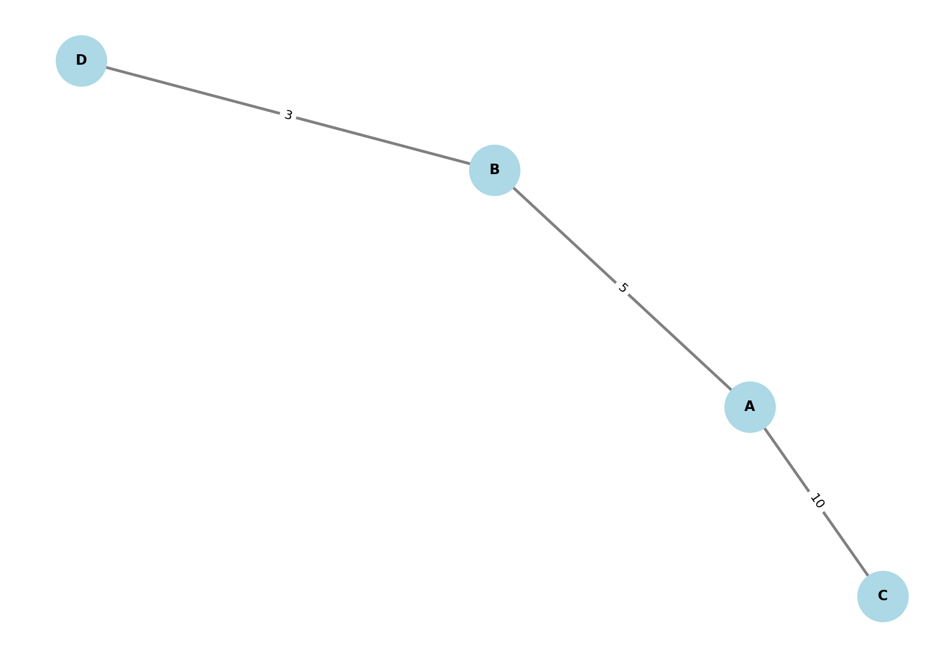
\includegraphics[width=0.8\textwidth]{pic/aboba}
        \caption{Пример визуализации графа}\label{fig:vis}
    \end{figure}


    \section{Список смежности Ia}

    \subsection{Условие:} для каждой вершины графа вывести её степень.

    \subsection{Реализация}

    \begin{minted}{text}
def get_vertex_degrees(self):
    """ Возвращает словарь со степенями всех вершин.
    Для ориентированного графа возвращает (входящая, исходящая, общая). """
    degrees = {}
    for v in self._adj_list:
        if not self.is_directed:
            degrees[v] = len(self._adj_list[v])
        else:
            out_degree = len(self._adj_list[v])
            in_degree = sum(1 for u in self._adj_list if v in self._adj_list[u])
            degrees[v] = {
                "in": in_degree,
                "out": out_degree,
                "total": in_degree + out_degree
            }
    return degrees
    \end{minted}

    Метод проходит по всем вершинам графа и вычисляет их степень в зависимости от его типа:

    \textbf{Для неориентированного графа:} Степень вершины определяется простым подсчетом количества ее соседей (длина словаря смежных вершин).

    \textbf{Для ориентированного графа:} Метод разделяет степени. Исходящая степень (out\_degree) вычисляется как количество соседей, к которым есть путь от текущей вершины. Входящая степень (in\_degree) рассчитывается путем прохода по всем вершинам графа и подсчета тех, которые ссылаются на текущую. Результат упаковывается во вложенный словарь.

    \subsection{Пример работы}

    Входные данные:
    \begin{minted}{json}
{
    "is_directed": false,
    "is_weighted": true,
    "adj_list": {
        "A": {"B": 5, "C": 10},
        "B": {"A": 5, "D": 3},
        "C": {"A": 10},
        "D": {"B": 3}
    }
}
    \end{minted}

    \begin{figure}[H]
        \centering
        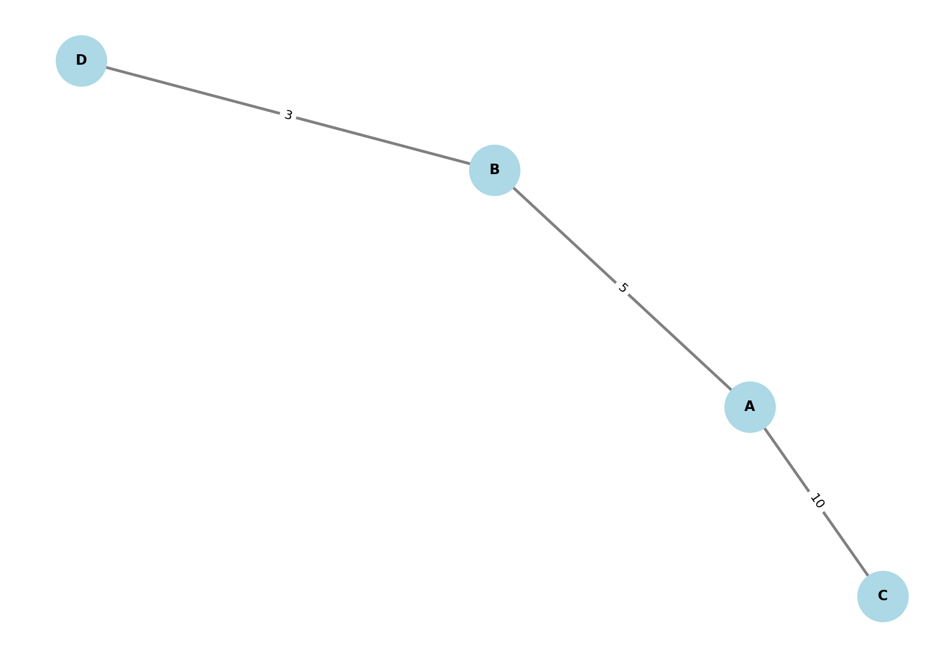
\includegraphics[width=0.8\textwidth]{pic/aboba}
    \end{figure}

    Вывод программы:
    \begin{minted}{text}
--- СТЕПЕНИ ВЕРШИН ---
Вершина A     | Степень: 2
Вершина B     | Степень: 2
Вершина C     | Степень: 1
Вершина D     | Степень: 1
    \end{minted}


    \section{Список смежности Ia}

    \subsection{Условие:} вывести все вершины графа, не смежные с данной

    \subsection{Реализация}
    \begin{minted}{text}
def get_non_adjacent_vertices(self, v: str):
    """ Возвращает список всех вершин, не смежных с данной вершиной v. """
    if v not in self._adj_list:
        raise GraphError(f"Вершина '{v}' не найдена в графе.")

    adjacent = set(self._adj_list[v].keys())

    non_adjacent = [
        node for node in self._adj_list
        if node != v and node not in adjacent
    ]
    return non_adjacent
    \end{minted}

    Метод использует эффективный подход для отсеивания соседей:

    \begin{enumerate}
        \item Сначала идет проверка на существование переданной вершины.
        \item Все смежные вершины сохраняются в структуру set.
        \item Затем с помощью генератора списков метод проходит по всем узлам графа и отбирает те, которые не являются самой исходной вершиной v и не входят в подготовленное множество смежных вершин.
    \end{enumerate}

    \subsection{Пример работы}

    Входные данные:
    \begin{minted}{json}
{
    "is_directed": false,
    "is_weighted": true,
    "adj_list": {
        "A": {"B": 5, "C": 10},
        "B": {"A": 5, "D": 3},
        "C": {"A": 10},
        "D": {"B": 3}
    }
}
    \end{minted}

    \begin{figure}[H]
        \centering
        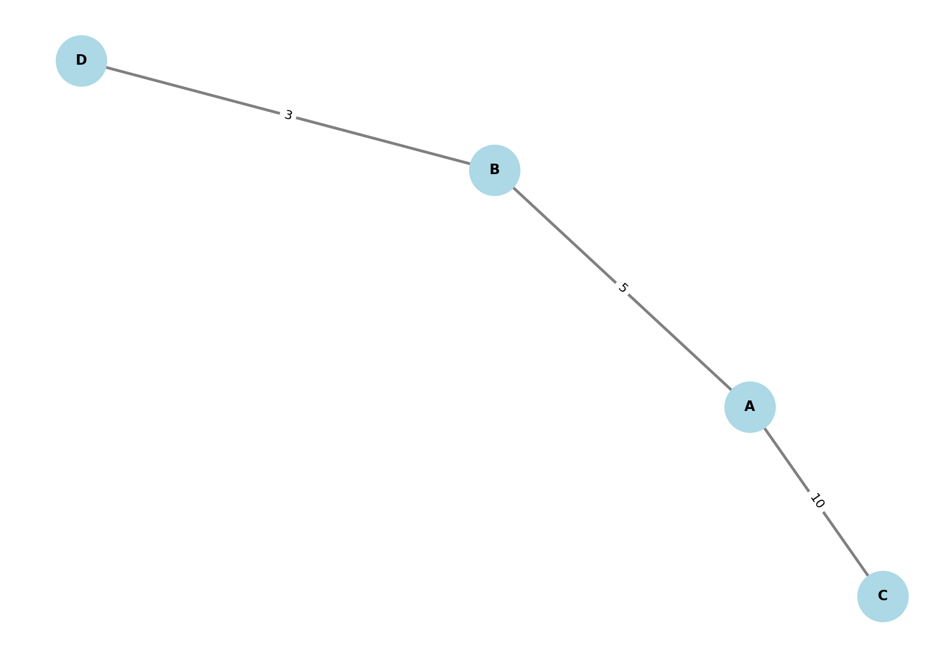
\includegraphics[width=0.8\textwidth]{pic/aboba}
    \end{figure}

    Вывод программы:
    \begin{minted}{text}
Введите имя целевой вершины: A
Вершины, не смежные с 'A': D
    \end{minted}


    \section{Список смежности Iб: несколько графов}

    \subsection{Условие:} построить орграф, являющийся объединением двух заданных

    \subsection{Реализация}

    \begin{minted}{text}
@classmethod
def union(cls, g1, g2):
    """ Построение объединения двух графов. """
    if g1.is_directed != g2.is_directed:
        raise GraphError("Нельзя объединить ориентированный и неориентированный графы.")

    new_is_weighted = g1.is_weighted or g2.is_weighted
    new_graph = cls(is_directed=g1.is_directed, is_weighted=new_is_weighted)

    for v in g1._adj_list:
        new_graph.add_vertex(v)
    for u, v, w in g1.get_edge_list():
        new_graph.add_edge(u, v, w)

    for v in g2._adj_list:
        if v not in new_graph._adj_list:
            new_graph.add_vertex(v)

    for u, v, w in g2.get_edge_list():
        if v in new_graph._adj_list[u]:
            current_weight = new_graph._adj_list[u][v]
            new_graph._adj_list[u][v] = current_weight + w
            if not new_graph.is_directed:
                new_graph._adj_list[v][u] = current_weight + w
        else:
            new_graph.add_edge(u, v, w)

    return new_graph
    \end{minted}

    Метод реализован через @classmethod, который создает новый объект графа на основе двух существующих:

    \begin{enumerate}
        \item \textbf{Проверка совместимости:} Графы можно объединить, только если у них совпадает флаг ориентированности. Результирующий граф будет взвешенным, если хотя бы один из исходных графов имел веса.
        \item \textbf{Перенос первого графа:} В новый граф полностью копируются все вершины и ребра из графа g1.
        \item \textbf{Добавление второго графа:} Вершины из g2 добавляются только если их еще нет в новом графе. При переносе ребер из g2 происходит проверка: если такое ребро уже существует, их веса суммируютс, а если нет — просто создается новое ребро.
    \end{enumerate}

    \subsection{Пример работы}

    Входные данные:

    Граф 1:
    \begin{minted}{json}
{
    "is_directed": false,
    "is_weighted": true,
    "adj_list": {
        "A": {"B": 5, "C": 10},
        "B": {"A": 5, "D": 3},
        "C": {"A": 10},
        "D": {"B": 3}
    }
}
    \end{minted}

    \begin{figure}[H]
        \centering
        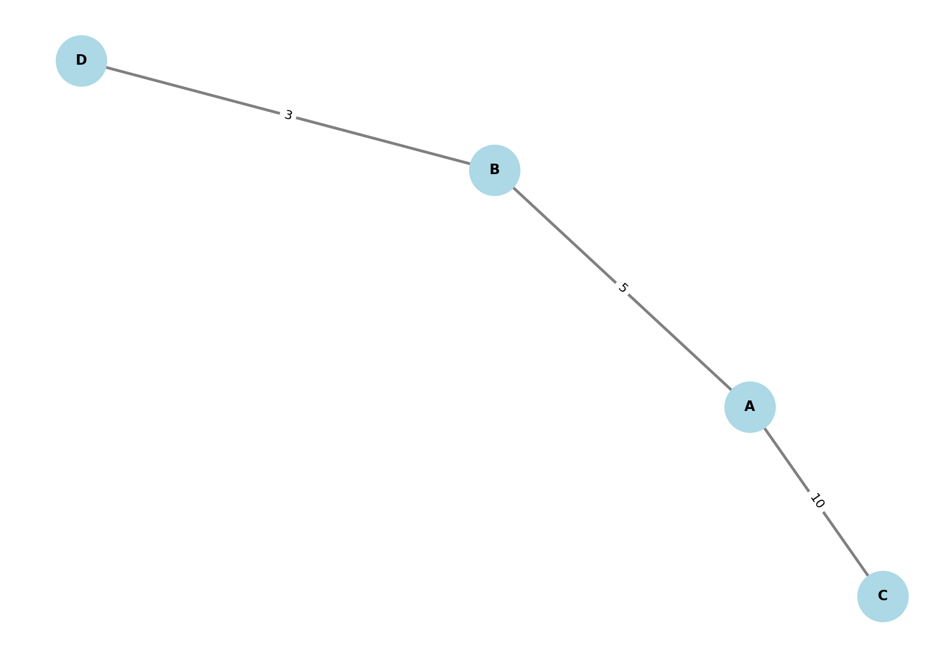
\includegraphics[width=0.8\textwidth]{pic/aboba}
    \end{figure}

    Граф 2:
    \begin{minted}{json}
{
    "is_directed": true,
    "is_weighted": true,
    "adj_list": {
        "S": {"A": 10, "C": 5},
        "A": {"B": 10, "D": 5},
        "B": {"T": 10},
        "C": {"B": 5},
        "D": {"T": 5},
        "T": {}
    }
}
    \end{minted}

    \begin{figure}[H]
        \centering
        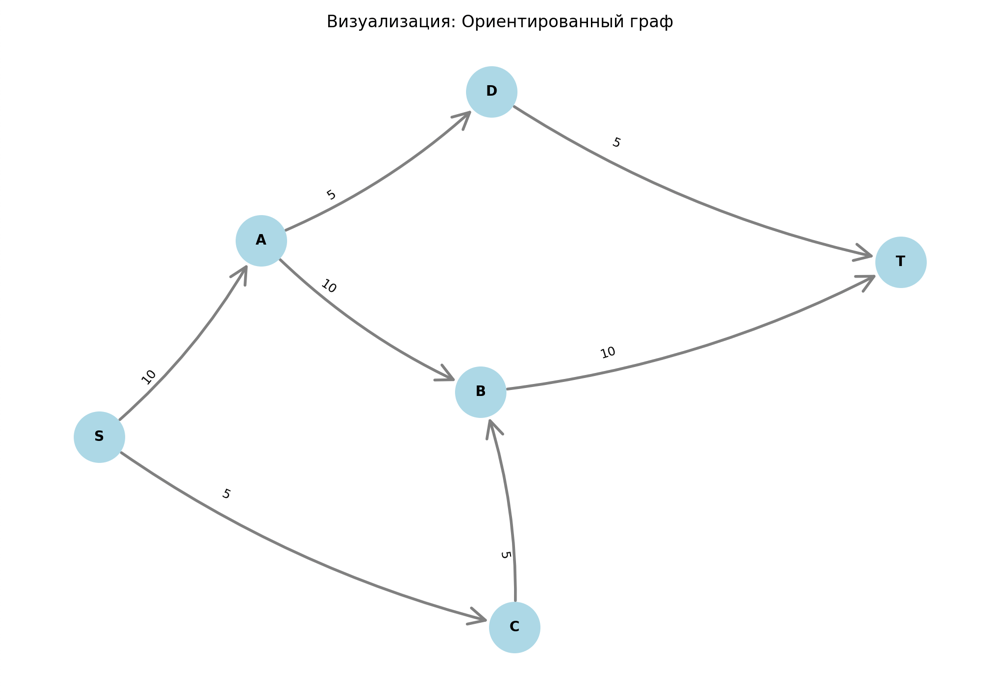
\includegraphics[width=0.8\textwidth]{pic/test}
    \end{figure}

    Вывод программы:
    \begin{minted}{text}
Введите имя первого JSON-файла: aboba
Введите имя второго JSON-файла: test
[ОШИБКА]: Нельзя объединить ориентированный и неориентированный графы.
    \end{minted}

    Граф 1:
    \begin{minted}{json}
{
    "is_directed": false,
    "is_weighted": true,
    "adj_list": {
        "A": {"B": 5, "C": 10},
        "B": {"A": 5, "D": 3},
        "C": {"A": 10},
        "D": {"B": 3}
    }
}
    \end{minted}

    \begin{figure}[H]
        \centering
        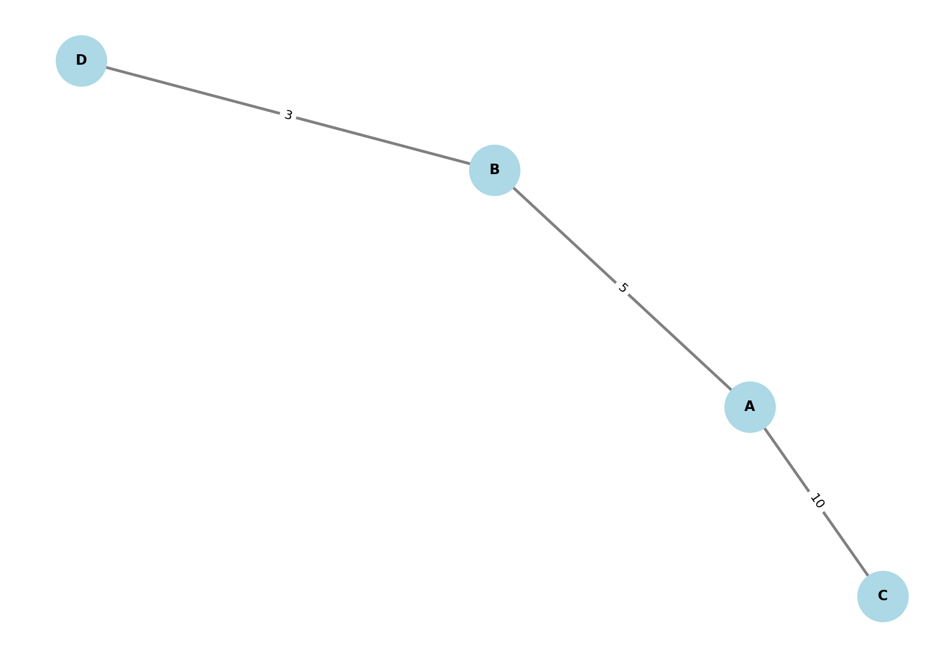
\includegraphics[width=0.8\textwidth]{pic/aboba}
    \end{figure}

    Граф 2:
    \begin{minted}{json}
{
    "is_directed": false,
    "is_weighted": true,
    "adj_list": {
        "a": {"b": 10.0},
        "b": {"a": 1},
        "c": {}
    }
}
    \end{minted}

    \begin{figure}[H]
        \centering
        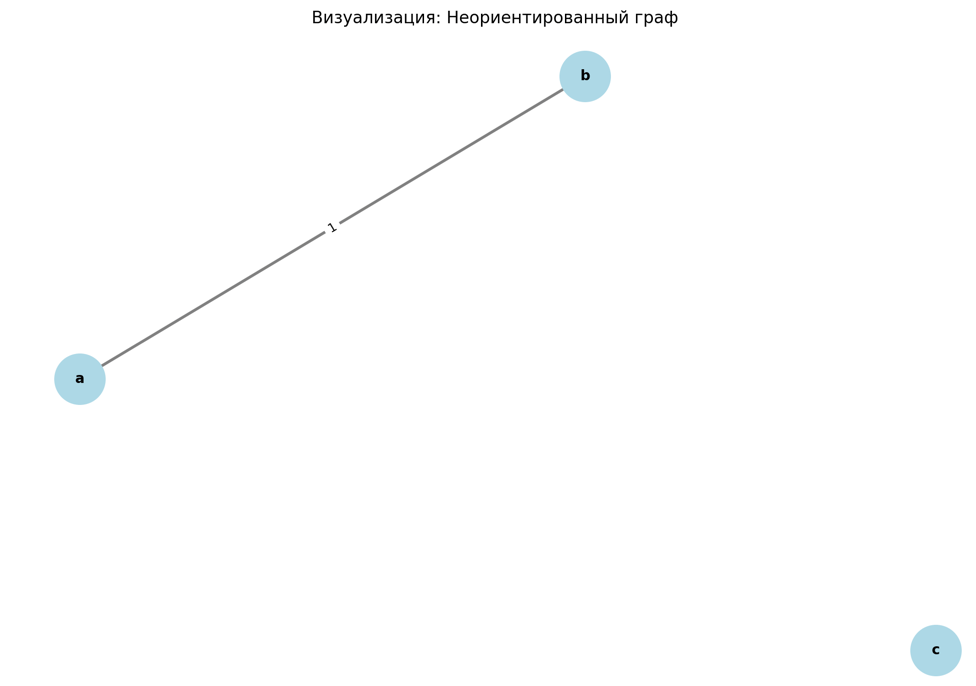
\includegraphics[width=0.8\textwidth]{pic/test2}
    \end{figure}

    Вывод программы:
    \begin{minted}{text}
Введите имя первого JSON-файла: aboba
Введите имя второго JSON-файла: test2

[УСПЕХ]: Графы из 'aboba' и 'test2' объединены.
Итого вершин: 7
    \end{minted}

    Итоговый граф:
    \begin{minted}{text}
A: B(5), C(10)
B: A(5), D(3)
C: A(10)
D: B(3)
a: b(10.0)
b: a(10.0)
c: -
    \end{minted}

    \begin{figure}[H]
        \centering
        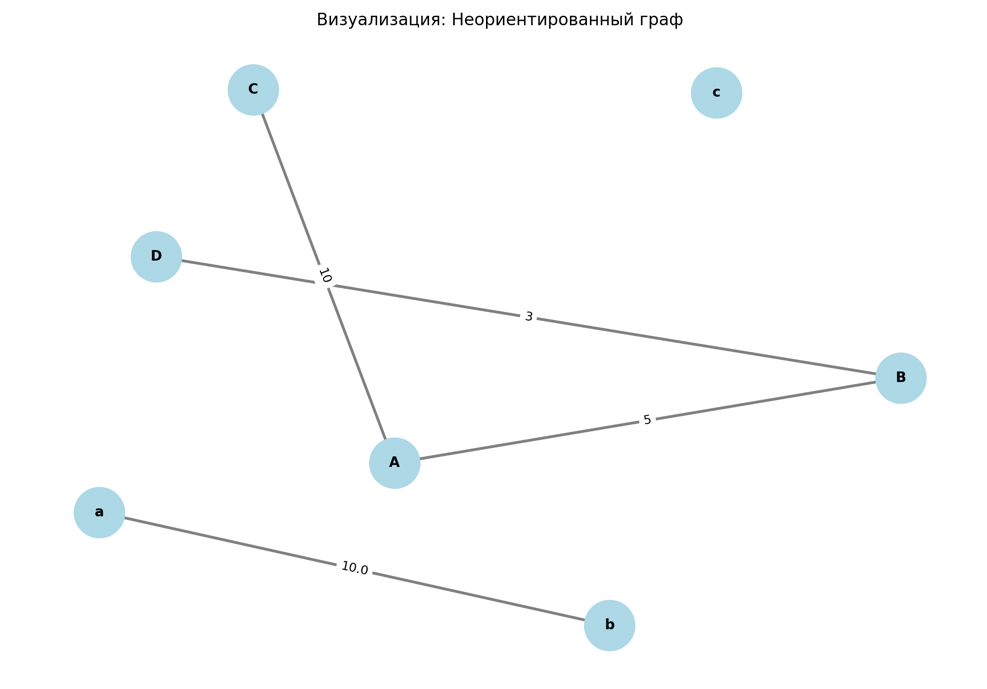
\includegraphics[width=0.8\textwidth]{pic/res}
    \end{figure}


    \section{Обходы графа II}

    \subsection{Условие:} Проверить, является ли орграф деревом, или лесом, или не является ни тем, ни другим.

    \subsection{Реализация}

    \begin{minted}{text}
def is_tree_or_forest(self):
    """ Проверяет, является ли орграф деревом, лесом или ни тем, ни другим. """
    if not self.is_directed:
        return "Метод предназначен только для ориентированных графов."

    vertices = list(self._adj_list.keys())
    if not vertices:
        return "Пустой граф можно считать лесом."

    degrees = self.get_vertex_degrees()
    for v in vertices:
        if degrees[v]['in'] > 1:
            return "Не является ни деревом, ни лесом (у вершины степень захода > 1)."

    visited = set()
    rec_stack = set()

    def has_cycle(v):
        visited.add(v)
        rec_stack.add(v)
        for neighbor in self._adj_list[v]:
            if neighbor not in visited:
                if has_cycle(neighbor):
                    return True
            elif neighbor in rec_stack:
                return True
        rec_stack.remove(v)
        return False

    for node in vertices:
        if node not in visited:
            if has_cycle(node):
                return "Не является ни деревом, ни лесом (содержит цикл)."

    roots = [v for v in vertices if degrees[v]['in'] == 0]

    if len(roots) == 1:
        return "дерево."
    elif len(roots) > 1:
        return "лес (несколько корней)."
    else:
        return "не является ни деревом, ни лесом."
    \end{minted}

    Метод определяет структуру ориентированного графа, последовательно проверяя соответствие его свойств теоретико-графовым определениям дерева и леса. Сначала осуществляется проверка входящих степеней: если существует хотя бы одна вершина, в которую входит более одного ребра, граф бракуется, поскольку в древовидных структурах каждый узел имеет не более одного родителя. Затем с помощью обхода в глубину алгоритм выявляет наличие циклов, сохраняя посещенные узлы и отслеживая текущий стек вызовов рекурсии. Если циклов не обнаружено, алгоритм подсчитывает количество корневых вершин, характеризующихся нулевой полустепенью захода. Наличие ровно одного корня означает, что структура является цельным деревом, тогда как несколько корней классифицируют граф как лес, состоящий из независимых деревьев.

    \subsection{Пример работы}

    Пример 1: граф - дерево:
    \begin{minted}{json}
{
    "is_directed": true,
    "is_weighted": false,
    "adj_list": {
        "A": {"B": 1.0, "C": 1.0},
        "B": {"D": 1.0, "E": 1.0},
        "C": {"F": 1.0},
        "D": {},
        "E": {},
        "F": {}
    }
}
    \end{minted}

    \begin{figure}[H]
        \centering
        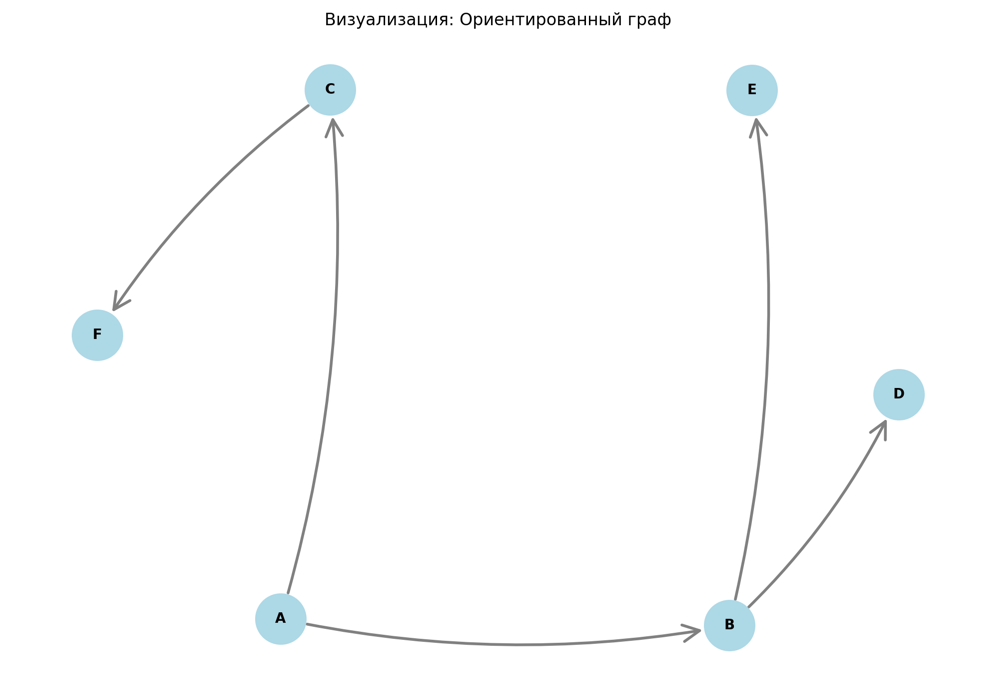
\includegraphics[width=0.8\textwidth]{pic/tree}
    \end{figure}

    Вывод программы:
    \begin{minted}{text}
Граф — дерево.
    \end{minted}

    Пример 2: граф - лес:
    \begin{minted}{json}
{
    "is_directed": true,
    "is_weighted": false,
    "adj_list": {
        "A": {"B": 1.0, "C": 1.0},
        "B": {},
        "C": {"D": 1.0},
        "D": {},
        "E": {"F": 1.0, "G": 1.0},
        "F": {},
        "G": {}
    }
}
    \end{minted}

    \begin{figure}[H]
        \centering
        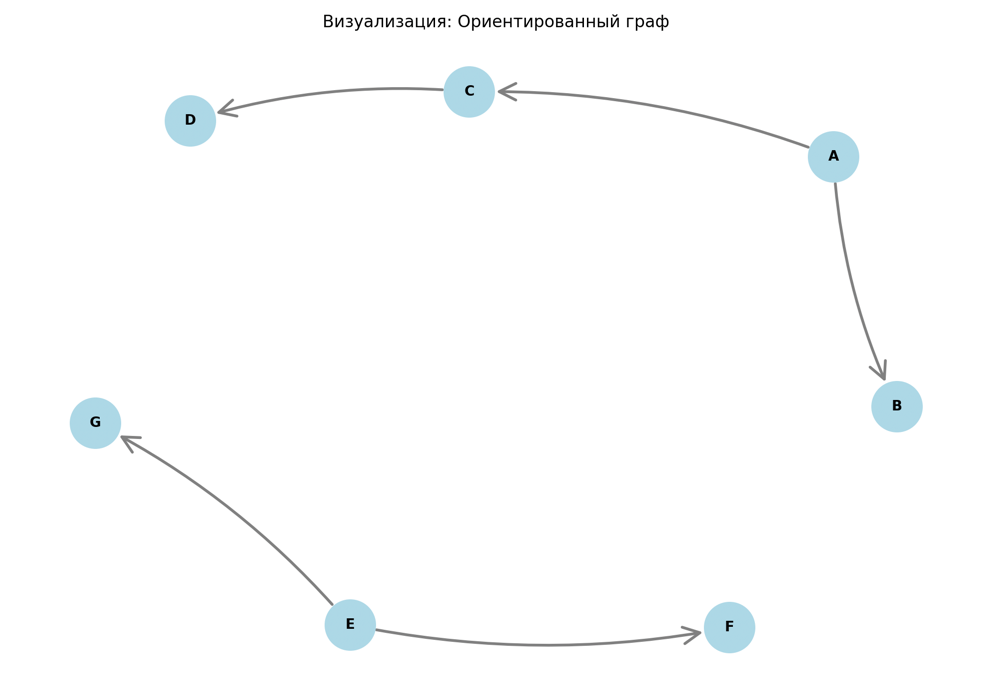
\includegraphics[width=0.8\textwidth]{pic/forest}
    \end{figure}

    Вывод программы:
    \begin{minted}{text}
Граф — лес (несколько корней).
    \end{minted}

    Пример 3: граф - ни лес, ни дерево:
    \begin{minted}{json}
{
    "is_directed": true,
    "is_weighted": true,
    "adj_list": {
        "A": {"B": 3, "C": 8},
        "B": {"C": 1, "D": 5},
        "C": {"D": 2},
        "D": {"A": 4}
    }
}
    \end{minted}

    \begin{figure}[H]
        \centering
        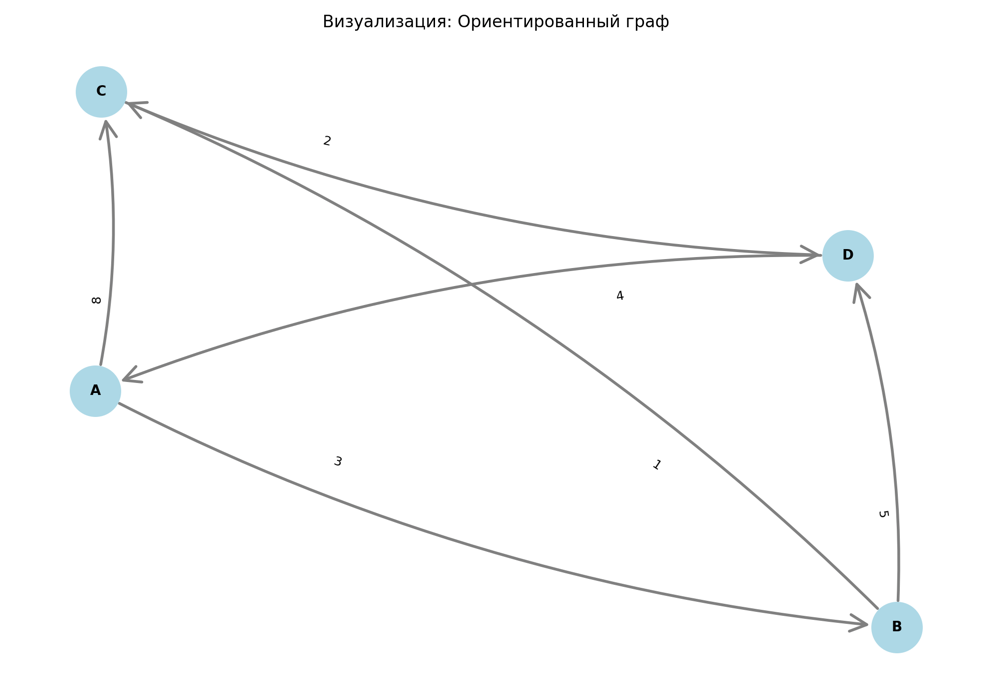
\includegraphics[width=0.8\textwidth]{pic/fl_test}
    \end{figure}

    Вывод программы:
    \begin{minted}{text}
Граф — Не является ни деревом, ни лесом (у вершины степень захода > 1).
    \end{minted}

    \section{Обходы графа II}

    \subsection{Условие:} Для каждой вершины найти кратчайшее (по числу рёбер) расстояние от неё до ближайшей из заданного множества вершин.

    \subsection{Реализация}

    \begin{minted}{text}
def find_shortest_to_set_universal(self, target_set: list) -> dict:
    """ Находит кратчайшее расстояние от каждой вершины до ближайшей из target_set. """

    for v in target_set:
        if v not in self._adj_list:
            raise GraphError(f"Вершина '{v}' не найдена.")

    distances = {v: float('inf') for v in self._adj_list}
    queue = deque()

    for v in target_set:
        distances[v] = 0
        queue.append(v)

    if self.is_directed:
        predecessors = {v: [] for v in self._adj_list}
        for u in self._adj_list:
            for v in self._adj_list[u]:
                predecessors[v].append(u)

    while queue:
        current_v = queue.popleft()

        neighbors = predecessors[current_v] if self.is_directed else self._adj_list[current_v]

        for neighbor in neighbors:
            if distances[neighbor] == float('inf'):
                distances[neighbor] = distances[current_v] + 1
                queue.append(neighbor)

    return distances
    \end{minted}

    Алгоритм вычисляет минимальные расстояния, опираясь на концепцию многоисточникового поиска в ширину. Изначально в очередь одновременно помещаются все целевые вершины, а расстояния до них принимаются равными нулю. Ключевой особенностью реализации для ориентированных графов является предварительное построение словаря предшественников. Это действие необходимо, поскольку требуется найти путь от произвольных вершин к целевым, что эквивалентно обходу графа в обратном направлении начиная от множества целей. В процессе извлечения узлов из очереди алгоритм однократно обновляет расстояния для всех непосещенных соседей, увеличивая текущее значение на единицу. Подобный подход гарантирует линейную сложность и корректное нахождение кратчайшего пути по количеству ребер.

    \subsection{Пример работы}

    \begin{minted}{json}
{
    "is_directed": true,
    "is_weighted": false,
    "adj_list": {
        "A": {"B": 1.0, "C": 1.0},
        "B": {"D": 1.0, "E": 1.0},
        "C": {"F": 1.0},
        "D": {},
        "E": {},
        "F": {}
    }
}
    \end{minted}

    \begin{figure}[H]
        \centering
        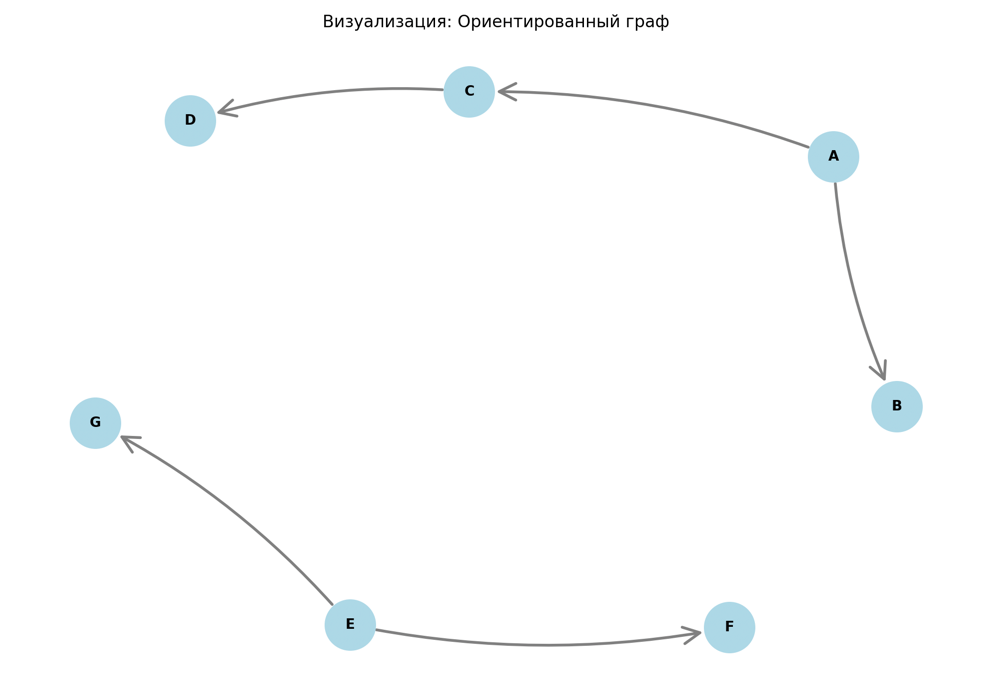
\includegraphics[width=0.8\textwidth]{pic/forest}
    \end{figure}

    Вывод программы:
    \begin{minted}{text}
Введите имена целевых вершин через пробел: E F

Кратчайшие расстояния до ближайшей из ['E', 'F']:
Вершина A          | Расстояние: 2
Вершина B          | Расстояние: 1
Вершина C          | Расстояние: 1
Вершина D          | Расстояние: inf
Вершина E          | Расстояние: 0
Вершина F          | Расстояние: 0
    \end{minted}

    \section{Каркас III}

    \subsection{Условие:} Дан взвешенный неориентированный граф из N вершин и M ребер. Требуется найти в нем каркас минимального веса. Использовать алгоритм Краскала.

    \subsection{Реализация}

    \begin{minted}{text}
def find_mst_kruskal(self):
    """ Находит минимальное остовное дерево (каркас) методом Краскала. """
    if self.is_directed:
        raise GraphError("Алгоритм Краскала предназначен для неориентированных графов.")
    if not self.is_weighted:
        raise GraphError("Для поиска MST граф должен быть взвешенным.")

    num_vertices = len(self._adj_list)
    if num_vertices == 0:
        return Graph(False, True), 0

    parent = {v: v for v in self._adj_list}
    rank = {v: 0 for v in self._adj_list}

    def find(v):
        if parent[v] == v:
            return v
        parent[v] = find(parent[v])
        return parent[v]

    def union(u, v):
        root_u = find(u)
        root_v = find(v)
        if root_u != root_v:
            if rank[root_u] < rank[root_v]:
                parent[root_u] = root_v
            elif rank[root_u] > rank[root_v]:
                parent[root_v] = root_u
            else:
                parent[root_v] = root_u
                rank[root_u] += 1
            return True
        return False

    edges = self.get_edge_list()
    edges.sort(key=lambda x: x[2])

    mst_graph = Graph(is_directed=False, is_weighted=True)
    for v in self._adj_list:
        mst_graph.add_vertex(v)

    edges_count = 0
    total_weight = 0

    for u, v, weight in edges:
        if edges_count == num_vertices - 1:
            break
        if find(u) != find(v):
            union(u, v)
            mst_graph.add_edge(u, v, weight)
            total_weight += weight
            edges_count += 1

    return mst_graph, total_weight
    \end{minted}

    Метод конструирует минимальное остовное дерево с помощью жадного алгоритма Краскала, дополненного структурой данных системы непересекающихся множеств. Для минимизации вычислительной сложности операций объединения компонентов и проверки принадлежности используются эвристики сжатия путей и ранжирования. На начальном этапе все связи графа извлекаются в единый список и сортируются по неубыванию их весовых коэффициентов. Далее алгоритм итеративно обрабатывает отсортированный список: если инцидентные ребру вершины принадлежат разным поддеревьям, то есть ребро не формирует цикл, оно включается в каркас, а соответствующие поддеревья сливаются воедино. Процесс оптимизирован и завершается досрочно, как только количество добавленных ребер становится строго на единицу меньше общего числа вершин графа.

    \subsection{Пример работы}

    \begin{minted}{json}
{
    "is_directed": false,
    "is_weighted": true,
    "adj_list": {
        "V1": {"V2": 6, "V3": 1, "V4": 5},
        "V2": {"V1": 6, "V3": 5, "V5": 3},
        "V3": {"V1": 1, "V2": 5, "V4": 5, "V5": 6, "V6": 4},
        "V4": {"V1": 5, "V3": 5, "V6": 2},
        "V5": {"V2": 3, "V3": 6, "V6": 6},
        "V6": {"V3": 4, "V4": 2, "V5": 6}
    }
}
    \end{minted}

    \begin{figure}[H]
        \centering
        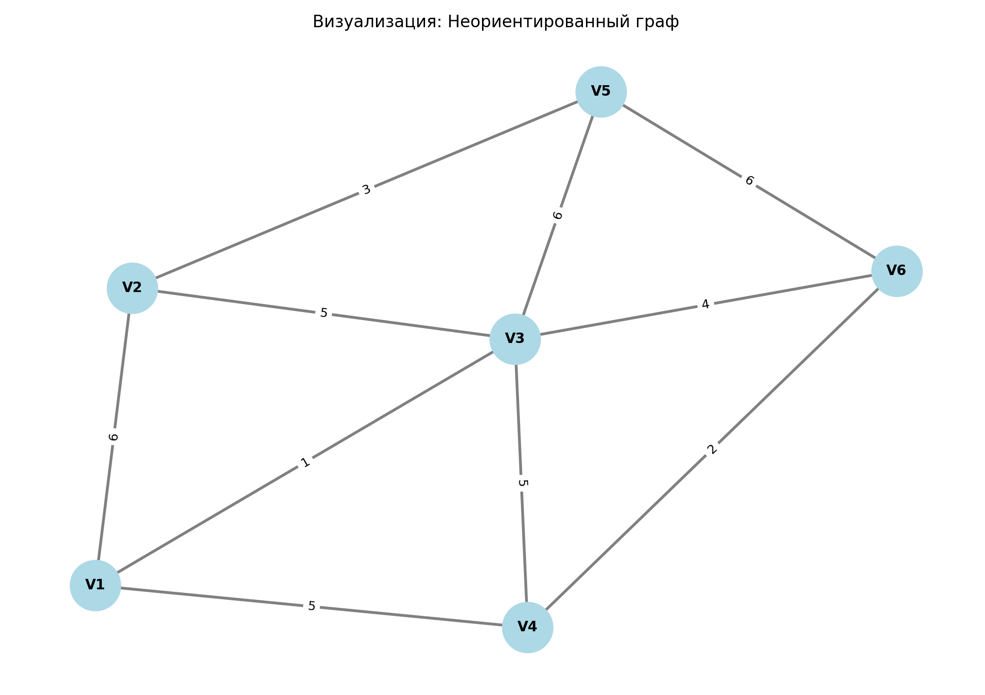
\includegraphics[width=0.8\textwidth]{pic/kr}
    \end{figure}

    Вывод программы:
    \begin{minted}{text}
Минимальный каркас найден!
Общий вес: 15.00
Результат: Остовное дерево
Ребра каркаса:
V1: V3(1)
V2: V5(3), V3(5)
V3: V1(1), V6(4), V2(5)
V4: V6(2)
V5: V2(3)
V6: V4(2), V3(4)
    \end{minted}

    \begin{figure}[H]
        \centering
        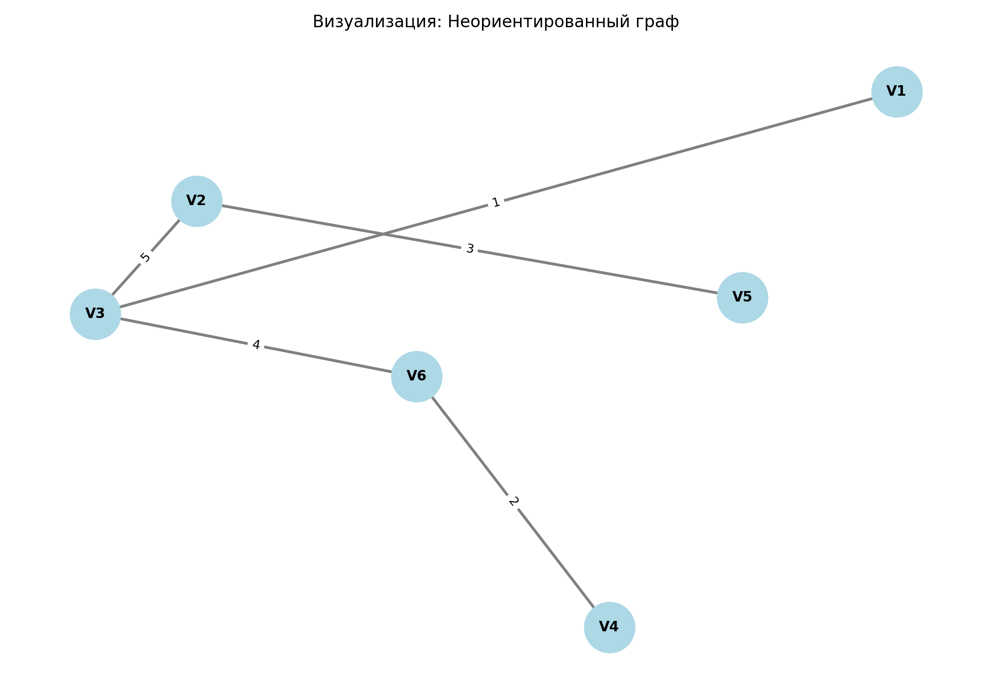
\includegraphics[width=0.8\textwidth]{pic/kr_vis}
    \end{figure}

    \section{Веса IV а}

    \subsection{Условие:} Найти k кратчайших путей между вершинами u и v.

    \subsection{Реализация}

    \begin{minted}{text}
def find_k_shortest_paths(self, start: str, end: str, k: int):
    """ Поиск k кратчайших путей между u и v (Алгоритм Йена + Дейкстра). """
    if start not in self._adj_list or end not in self._adj_list:
        raise GraphError("Вершины не найдены")

    def dijkstra(temp_graph, start, end):
        distances = {node: float('inf') for node in temp_graph._adj_list}
        distances[start] = 0
        paths = {node: [] for node in temp_graph._adj_list}
        paths[start] = [start]
        pq = [(0, start)]

        visited = set()
        while pq:
            (dist, current) = heapq.heappop(pq)
            if current in visited:
                continue
            if current == end:
                return (dist, paths[end])
            visited.add(current)

            for neighbor, weight in temp_graph._adj_list[current].items():
                if neighbor in visited:
                    continue

                new_dist = dist + weight
                if new_dist < distances[neighbor]:
                    distances[neighbor] = new_dist
                    paths[neighbor] = paths[current] + [neighbor]
                    heapq.heappush(pq, (new_dist, neighbor))
        return None

    A = []
    B = []

    initial_path = dijkstra(self, start, end)
    if not initial_path: return []
    A.append(initial_path)

    for i in range(1, k):
        for j in range(len(A[-1][1]) - 1):
            spur_node = A[-1][1][j]
            root_path = A[-1][1][:j + 1]

            edges_removed = []
            for path_data in A:
                path = path_data[1]
                if len(path) > j and root_path == path[:j + 1]:
                    u, v = path[j], path[j + 1]
                    if v in self._adj_list[u]:
                        weight = self._adj_list[u][v]
                        edges_removed.append((u, v, weight))
                        self.remove_edge(u, v)

            spur_path_data = dijkstra(self, spur_node, end)
            if spur_path_data:
                total_path = root_path[:-1] + spur_path_data[1]
                total_dist = sum(self.get_edge_weight(total_path[m], total_path[m + 1])
                                 for m in range(len(total_path) - 1))
                if (total_dist, total_path) not in B:
                    heapq.heappush(B, (total_dist, total_path))

            for u, v, w in edges_removed:
                self.add_edge(u, v, w)

        if not B: break
        A.append(heapq.heappop(B))

    return A

def get_edge_weight(self, u, v):
    return self._adj_list[u][v]
    \end{minted}

    Алгоритм Йена вычисляет заданное количество кратчайших путей, опираясь на классический алгоритм Дейкстры в качестве базовой подпрограммы. На первом этапе определяется абсолютно кратчайший маршрут между исходной и целевой вершинами. Далее алгоритм итеративно строит альтернативные варианты (отклонения), рассматривая каждую вершину текущего пути как точку ветвления. Чтобы гарантировать нахождение новых, независимых маршрутов, ребра, принадлежащие уже найденным путям на совпадающих участках, временно исключаются из графа. Найденные пути-кандидаты сохраняются в приоритетную очередь, из которой на каждой итерации извлекается минимальный по весу маршрут, пополняя итоговый список кратчайших путей.

    \subsection{Пример работы}

    \begin{minted}{json}
{
    "is_directed": true,
    "is_weighted": true,
    "adj_list": {
        "A": {"C": 4, "E": 10},
        "B": {"A": 1, "C": 2, "E": 8},
        "C": {"E": 3},
        "D": {"A": 3, "B": 2},
        "E": {}
    }
}
    \end{minted}

    \begin{figure}[H]
        \centering
        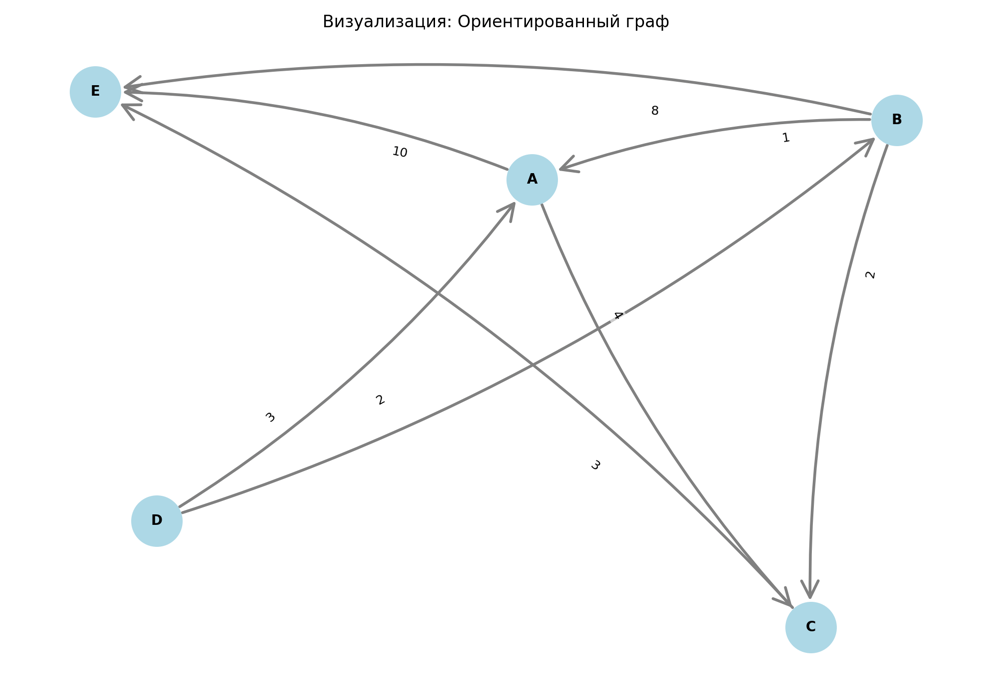
\includegraphics[width=0.8\textwidth]{pic/yen}
    \end{figure}

    Вывод программы:
    \begin{minted}{text}
Начальная вершина: A
Конечная вершина: E
Количество путей (k): 3

Найдено 2 кратчайших путей:
1. Путь: A -> C -> E | Вес: 7.00
2. Путь: A -> E | Вес: 10.00
    \end{minted}

    \section{Веса IV b}

    \subsection{Условие:} Вывести кратчайшие пути для всех пар вершин.

    \subsection{Реализация}

    \begin{minted}{text}
def all_pairs_shortest_paths_floyd(self):
    """ Поиск кратчайших путей для всех пар вершин (Алгоритм Флойда-Уоршелла). """
    nodes = list(self._adj_list.keys())
    dist = {u: {v: float('inf') for v in nodes} for u in nodes}

    for u in nodes:
        dist[u][u] = 0
        for v, weight in self._adj_list[u].items():
            dist[u][v] = weight

    for k in nodes:
        for i in nodes:
            for j in nodes:
                if dist[i][j] > dist[i][k] + dist[k][j]:
                    dist[i][j] = dist[i][k] + dist[k][j]
    return dist
    \end{minted}

    Решение задачи поиска кратчайших путей между всеми парами вершин реализовано посредством алгоритма Флойда-Уоршелла, который базируется на парадигме динамического программирования. Изначально формируется матрица смежности, где расстояния между напрямую связанными узлами равны весам их ребер, а остальные инициализируются бесконечностью. Затем алгоритм использует три вложенных цикла для последовательной проверки каждой вершины графа в качестве возможной промежуточной точки. Если выясняется, что маршрут от начальной до конечной вершины через выбранный промежуточный узел короче, чем текущий известный путь, значение в матрице расстояний обновляется.

    \subsection{Пример работы}

    \begin{minted}{json}
{
    "is_directed": true,
    "is_weighted": true,
    "adj_list": {
        "A": {"B": 3, "C": 8},
        "B": {"C": 1, "D": 5},
        "C": {"D": 2},
        "D": {"A": 4}
    }
}
    \end{minted}

    \begin{figure}[H]
        \centering
        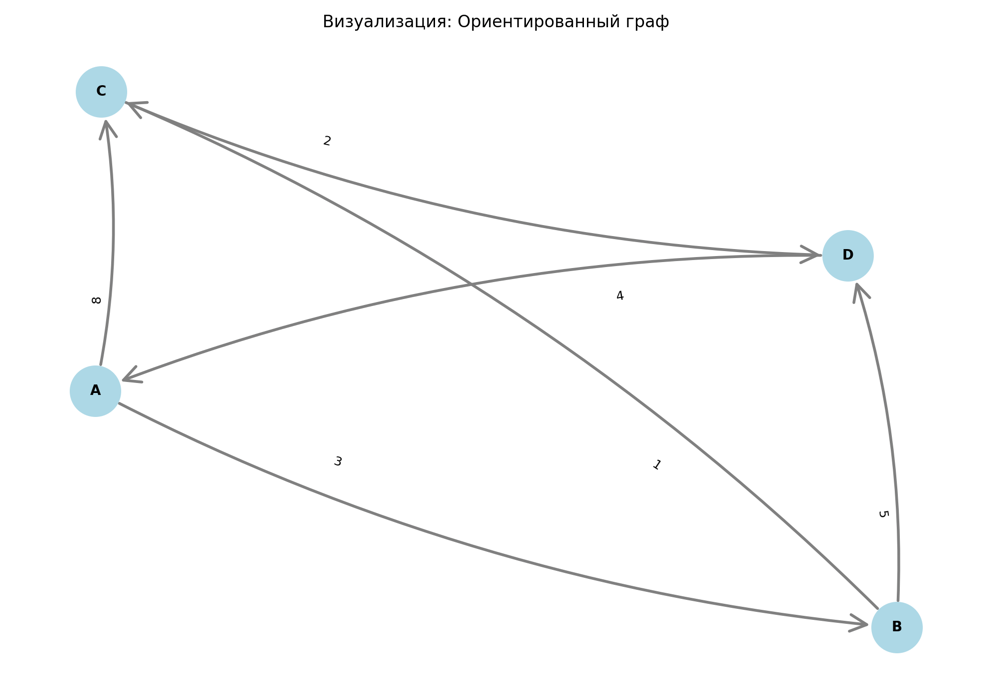
\includegraphics[width=0.8\textwidth]{pic/fl_test}
    \end{figure}

    Вывод программы:
    \begin{minted}{text}
--- МАТРИЦА КРАТЧАЙШИХ ПУТЕЙ (Флойд-Уоршелл) ---
          A         B         C         D
--------------------------------------------------
A         0.0       3.0       4.0       6.0
B         9.0       0.0       1.0       3.0
C         6.0       9.0       0.0       2.0
D         4.0       7.0       8.0       0.0
    \end{minted}

    \section{Веса IV с}

    \subsection{Условие:} Найти все такие пары вершин, что между ними существует путь сколько угодно малой длины.

    \subsection{Реализация}

    \begin{minted}{text}
def find_negative_cycle_pairs_bellman(self):
    """ Поиск всех пар вершин, между которыми существует путь сколь угодно малой длины.
     (Алгоритм Беллмана-Форда для поиска отрицательных циклов). """
    nodes = list(self._adj_list.keys())
    inf_paths = []

    for start_node in nodes:
        dist = {node: float('inf') for node in nodes}
        dist[start_node] = 0

        for _ in range(len(nodes) - 1):
            for u, v, w in self.get_edge_list():
                if dist[u] != float('inf') and dist[u] + w < dist[v]:
                    dist[v] = dist[u] + w

        affected_by_cycle = set()
        for _ in range(len(nodes)):
            for u, v, w in self.get_edge_list():
                if dist[u] != float('inf') and dist[u] + w < dist[v]:
                    dist[v] = float('-inf')
                    affected_by_cycle.add(v)

        for target_node in nodes:
            if dist[target_node] == float('-inf'):
                inf_paths.append((start_node, target_node))

    return list(set(inf_paths))
    \end{minted}

    Для обнаружения путей бесконечно малой длины применяется расширенная версия алгоритма Беллмана-Форда, адаптированная для работы с циклами отрицательного веса. Метод запускается для каждой вершины графа, выполняя стандартную процедуру релаксации всех ребер заданное количество раз, что позволяет найти минимальные расстояния. После этого проводится дополнительная серия итераций: если расстояние до какой-либо вершины продолжает уменьшаться, это свидетельствует о ее достижимости из отрицательного цикла. Таким узлам принудительно присваивается бесконечно малое расстояние, и алгоритм фиксирует пары вершин, для которых итоговая стоимость пути устремляется в минус бесконечность.

    \subsection{Пример работы}

    \begin{minted}{json}
{
    "is_directed": true,
    "is_weighted": true,
    "adj_list": {
        "A": {"B": 5},
        "B": {"C": 2, "D": 3},
        "C": {"D": -10},
        "D": {"B": 1, "E": 3},
        "E": {}
    }
}
    \end{minted}

    \begin{figure}[H]
        \centering
        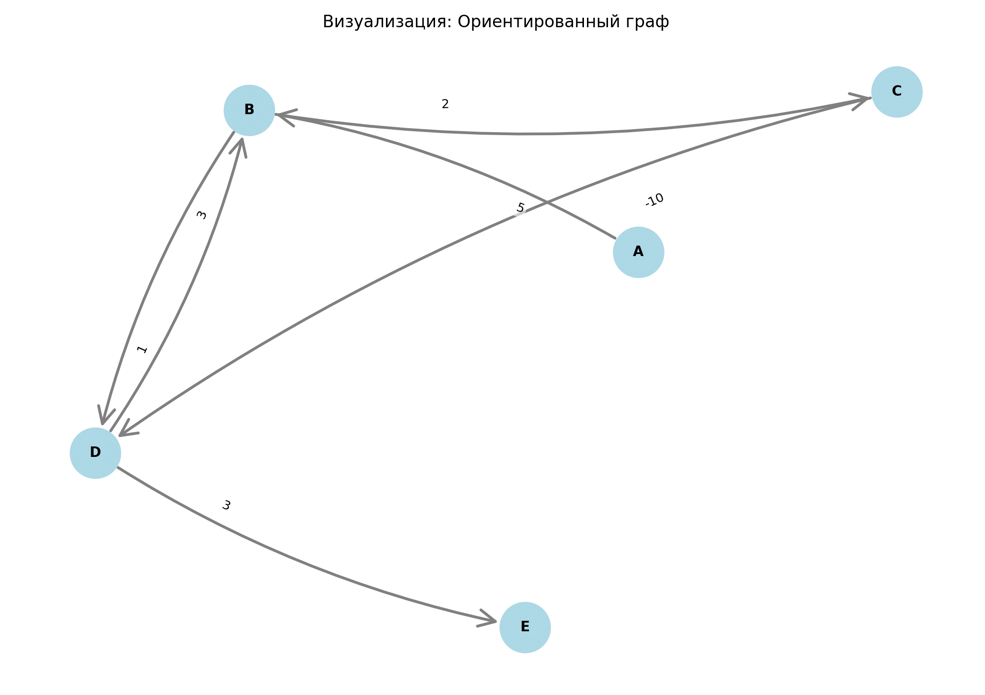
\includegraphics[width=0.8\textwidth]{pic/neg}
    \end{figure}

    Вывод программы:
    \begin{minted}{text}
Проверка бесконечно малых весов...
Обнаружены пути, проходящие через отрицательные циклы:
    Из вершины 'A' пути к узлам E, D, C, B проходят через отрицательные циклы
    Из вершины 'B' пути к узлам C, D, B, E проходят через отрицательные циклы
    Из вершины 'D' пути к узлам C, D, B, E проходят через отрицательные циклы
    Из вершины 'C' пути к узлам B, E, C, D проходят через отрицательные циклы
    \end{minted}

    \section{Максимальный поток V}

    \subsection{Условие:} Решить задачу на нахождение максимального потока любым алгоритмом.

    \subsection{Реализация}

    \begin{minted}{text}
def find_max_flow(self, source: str, sink: str):
    """Находит максимальный поток из истока в сток (Алгоритм Эдмондса-Карпа)."""
    if source not in self._adj_list or sink not in self._adj_list:
        raise GraphError("Указанные вершины истока или стока не найдены.")

    residual_adj = {u: {} for u in self._adj_list}
    for u in self._adj_list:
        for v, weight in self._adj_list[u].items():
            residual_adj[u][v] = weight
            if u not in residual_adj[v]:
                residual_adj[v][u] = 0

    max_flow = 0
    parent = {}
    all_paths = []

    def bfs():
        visited = {node: False for node in residual_adj}
        queue = deque([source])
        visited[source] = True
        while queue:
            u = queue.popleft()
            for v, capacity in residual_adj[u].items():
                if not visited[v] and capacity > 0:
                    parent[v] = u
                    visited[v] = True
                    if v == sink:
                        return True
                    queue.append(v)
        return False

    while bfs():
        path = []
        path_flow = float('inf')
        s = sink
        while s != source:
            path.append(s)
            path_flow = min(path_flow, residual_adj[parent[s]][s])
            s = parent[s]
        path.append(source)
        path.reverse()

        edges_info = []
        for i in range(len(path) - 1):
            u, v = path[i], path[i + 1]
            is_reverse = False
            if v not in self._adj_list.get(u, {}):
                is_reverse = True
            edges_info.append(f"{u}→{v} {'(обратная дуга)' if is_reverse else '(прямая)'}")

        all_paths.append((path.copy(), path_flow, edges_info.copy()))

        max_flow += path_flow
        v = sink
        while v != source:
            u = parent[v]
            residual_adj[u][v] -= path_flow
            residual_adj[v][u] += path_flow
            v = parent[v]

    return max_flow, all_paths
    \end{minted}

    Нахождение максимального потока осуществляется с помощью алгоритма Эдмондса-Карпа, который является эффективной реализацией метода Форда-Фалкерсона. Первоначально строится остаточная сеть, учитывающая как прямые пропускные способности, так и потенциальные обратные потоки. Для поиска увеличивающих путей от истока к стоку используется поиск в ширину (BFS), гарантирующий выбор маршрута с наименьшим числом ребер. Найдя такой путь, алгоритм определяет его узкое место (минимальную доступную пропускную способность), после чего обновляет веса в остаточной сети, вычитая найденное значение из прямых дуг и прибавляя к обратным. Процесс накопления максимального потока продолжается до тех пор, пока поиск в ширину способен достичь стока.

    \subsection{Пример работы}

    \begin{minted}{json}
{
    "is_directed": true,
    "is_weighted": true,
    "adj_list": {
        "S": {"A1": 10, "A2": 10},
        "A1": {"B1": 10, "B2": 10},
        "A2": {"B1": 10},
        "B1": {"T": 10},
        "B2": {"T": 10},
        "T": {}
    }
}
    \end{minted}

    \begin{figure}[H]
        \centering
        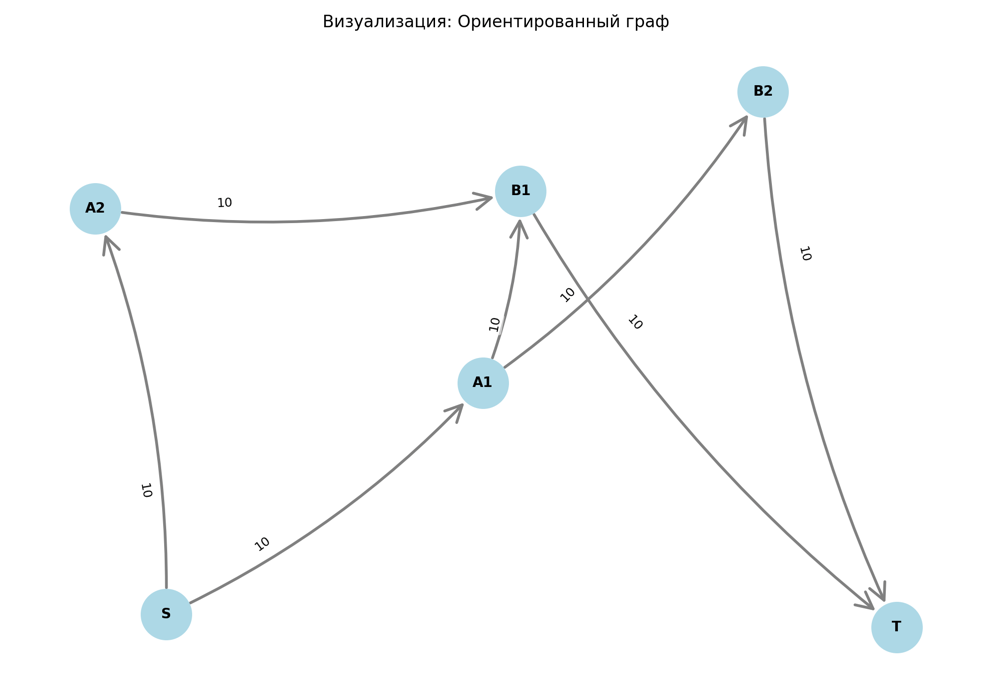
\includegraphics[width=0.8\textwidth]{pic/back}
    \end{figure}

    Вывод программы:
    \begin{minted}{text}
Введите исток: S
Введите сток: T

Итерация 1:
Путь: S → A1 → B1 → T (добавлен поток: 10)
Ребра: S→A1 (прямая), A1→B1 (прямая), B1→T (прямая)

Итерация 2:
Путь: S → A2 → B1 → A1 → B2 → T (добавлен поток: 10)
Ребра: S→A2 (прямая), A2→B1 (прямая), B1→A1 (обратная дуга), A1→B2 (прямая), B2→T (прямая)

Максимальный поток из S в T: 20
    \end{minted}

    \section{Творческое задание XII: Умная маршрутизация с применением ML}
    \subsection{Условие:} реализовать систему динамической маршрутизации, которая адаптирует веса рёбер графа (время в пути) на основе внешних факторов. Требуется построить предсказательную модель машинного обучения для оценки загруженности дорог в зависимости от времени суток, типа дня и погодных условий, а затем использовать эти предсказания для нахождения оптимальных маршрутов и визуализации пробок.

    \subsection{Реализация:}

    Основа системы — интеграция классических графовых алгоритмов (поиск k-кратчайших путей алгоритмом Йена) с предиктивной аналитикой.

    \begin{enumerate}
        \item \textbf{ML-составляющая:} За предсказание трафика отвечает класс TrafficPredictor, использующий модель градиентного бустинга GradientBoostingRegressor из библиотеки scikit-learn. Чтобы модель корректно воспринимала цикличность времени (например, что 23:00 и 01:00 находятся рядом), применяется синусно-косинусное преобразование часов. Также в качестве признаков выступают тип дня (будни/выходные), погодные условия (ясно/дождь/снег) и базовый вес ребра.





        \item \textbf{Динамический граф:} В API (FastAPI) реализована функция get\_effective\_graph, которая перед каждым поиском пути создает глубокую копию текущего графа и обновляет веса его рёбер на основе свежих предсказаний ML-модели. Это позволяет алгоритму Йена находить маршруты в обход «пробок».





        \item \textbf{Визуализация:} Пользовательский интерфейс на Streamlit позволяет гибко менять погодные и временные условия, после чего граф перерисовывается: рёбра с высокой предсказанной загрузкой (более 50\%) подсвечиваются красным цветом, со средней — желтым, а свободные дороги — синим.





    \end{enumerate}
    \textbf{Ключевые фрагменты кода:}

    Извлечение признаков и подготовка данных для модели машинного обучения:

    \begin{minted}{text}
def _extract_features(self, hour: int, day_type: int, weather: int, base_weight: float):
    # Циклическое кодирование времени суток (чтобы 23:00 и 00:00 были близки)
    hour_sin = np.sin(2 * np.pi * hour / 24)
    hour_cos = np.cos(2 * np.pi * hour / 24)

    return np.array([
        hour_sin,
        hour_cos,
        day_type,
        weather,
        base_weight,
        hour * day_type,   # Взаимодействие признаков (полиномиальные фичи)
        hour * weather
    ])
    \end{minted}


    Наложение предсказаний модели на веса графа перед маршрутизацией:

    \begin{minted}{text}
def get_effective_graph() -> Graph:
    """Возвращает граф с учетом трафика (если есть предсказания) или базовый граф."""
    if not latest_traffic_predictions:
        return current_graph

    # Создаем копию, чтобы не портить исходные базовые веса графа
    g = Graph.from_copy(current_graph)
    for (u, v), data in latest_traffic_predictions.items():
        try:
            # Заменяем вес на актуальный (предсказанный моделью)
            g.change_weight(u, v, data['current'])
            if not g.is_directed and v in g._adj_list and u in g._adj_list[v]:
                g._adj_list[v][u] = data['current']
        except:
            pass
    return g
    \end{minted}


    Модель обучается на синтетических паттернах трафика, где учитываются часы пик (7-9 и 17-19 часов в будние дни), снижение трафика ночью, а также штрафы за плохие погодные условия. В результате алгоритм поиска пути динамически подстраивается под ситуацию, отдавая предпочтение более длинным (по базовому весу), но свободным дорогам, если основные магистрали перегружены.

    \begin{figure}[H]
        \centering
        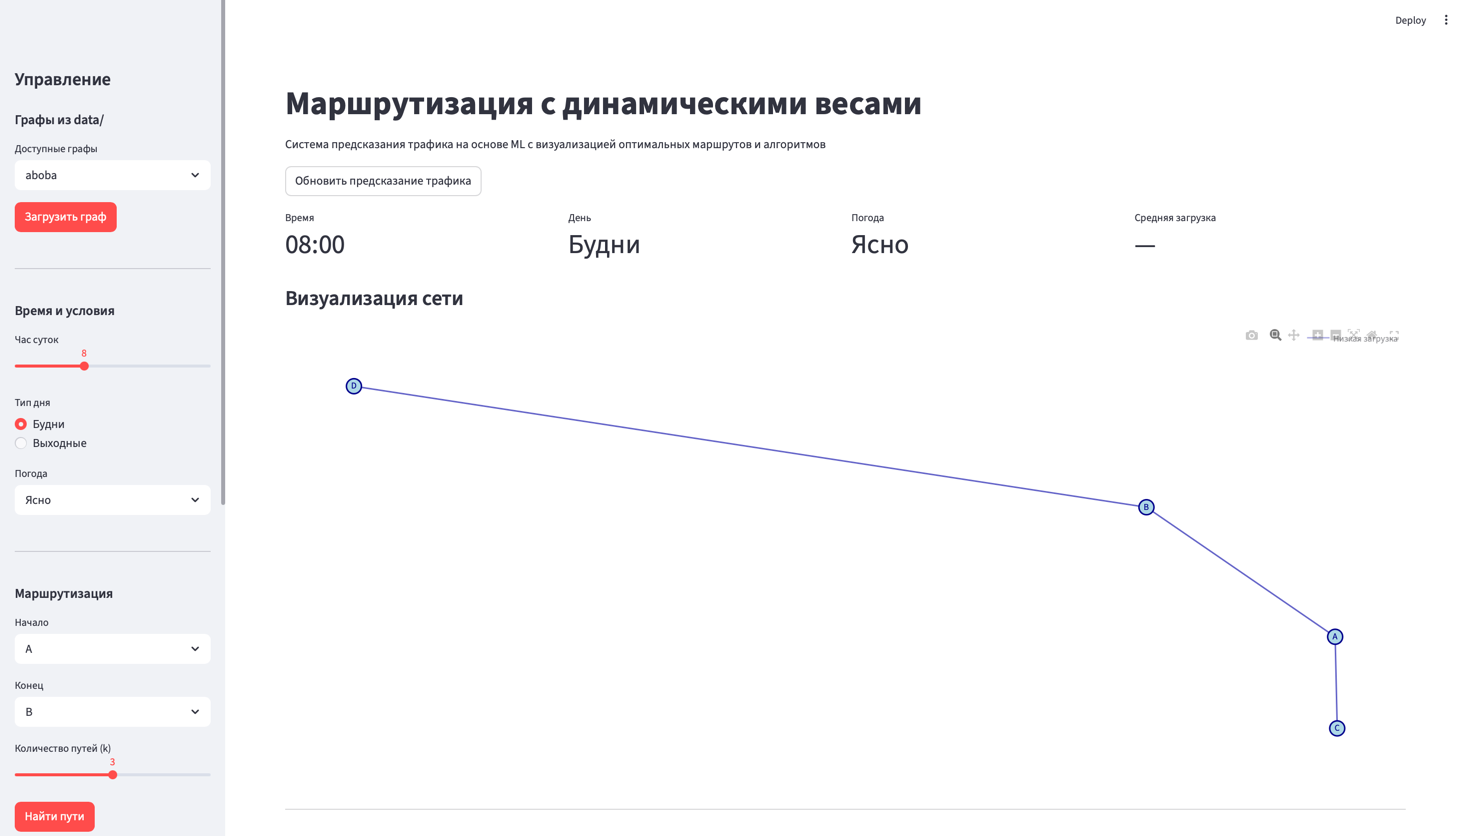
\includegraphics[width=0.8\textwidth]{pic/interface}
    \end{figure}
% Отобразить все источники. Даже те, на которые нет ссылок.
%    \nocite{*}
%
%    \bibliographystyle{ugost2003}
%    \bibliography{thesis}
%
%    \appendix

\end{document}